\documentclass[border=10pt]{standalone}
\usepackage[T1]{fontenc}
\usepackage{tikz}
\usetikzlibrary{positioning, arrows.meta, calc}

\definecolor{accent}{HTML}{1E3A8A}
\definecolor{boxfill}{HTML}{F1F5F9}
\definecolor{boxstroke}{HTML}{475569}

\begin{document}
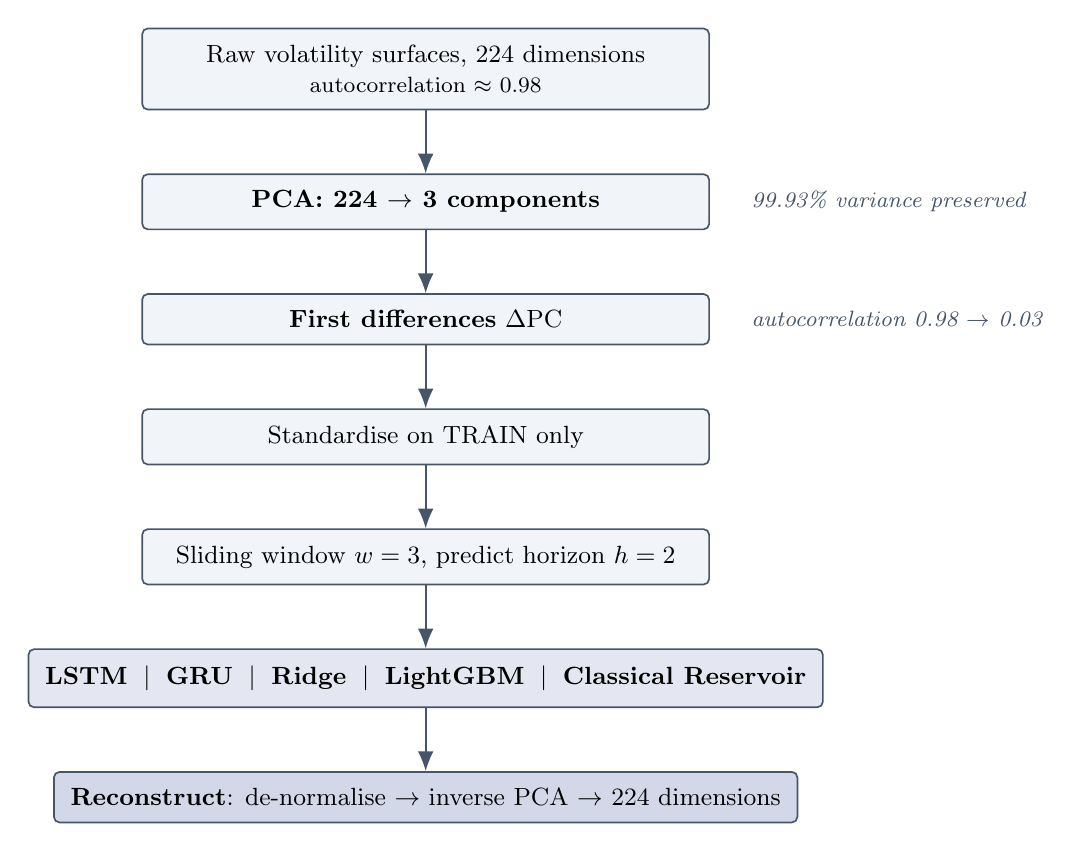
\begin{tikzpicture}[
  every node/.style={font=\small},
  >={Latex[length=2.5mm, width=2mm]},
  box/.style={
    draw=boxstroke, line width=0.6pt, fill=boxfill,
    rounded corners=2pt, inner sep=6pt,
    minimum width=72mm, align=center
  },
  modelbox/.style={
    draw=boxstroke, line width=0.6pt, fill=accent!12,
    rounded corners=2pt, inner sep=6pt,
    minimum width=72mm, align=center
  },
  note/.style={font=\footnotesize\itshape, color=boxstroke},
  arrow/.style={->, line width=0.6pt, draw=boxstroke}
]

\node[box] (raw) {Raw volatility surfaces, 224 dimensions \\ \footnotesize autocorrelation $\approx$ 0.98};
\node[box, below=8mm of raw] (pca) {\textbf{PCA: 224 $\rightarrow$ 3 components}};
\node[note, right=4mm of pca] {99.93\% variance preserved};

\node[box, below=8mm of pca] (diff) {\textbf{First differences} $\Delta\mathrm{PC}$};
\node[note, right=4mm of diff] {autocorrelation 0.98 $\rightarrow$ 0.03};

\node[box, below=8mm of diff] (std) {Standardise on TRAIN only};

\node[box, below=8mm of std] (window) {Sliding window $w=3$, predict horizon $h=2$};

\node[modelbox, below=8mm of window] (models) {\textbf{LSTM} $\;|\;$ \textbf{GRU} $\;|\;$ \textbf{Ridge} $\;|\;$ \textbf{LightGBM} $\;|\;$ \textbf{Classical Reservoir}};

\node[box, below=8mm of models, fill=accent!20] (rec) {\textbf{Reconstruct}: de-normalise $\rightarrow$ inverse PCA $\rightarrow$ 224 dimensions};

\draw[arrow] (raw) -- (pca);
\draw[arrow] (pca) -- (diff);
\draw[arrow] (diff) -- (std);
\draw[arrow] (std) -- (window);
\draw[arrow] (window) -- (models);
\draw[arrow] (models) -- (rec);

\end{tikzpicture}
\end{document}
